\chapter*{Übung 11}

\section*{Aufgabe 23}

Zur Erinnerung: $\beta_v = \frac{v}{c}$ und $\gamma_v = \frac{1}{\sqrt{1 - \beta_v^2}}$.

Nun soll mit einem beliebigen Vierervektor $x$ gelten: $\Lambda(v') x = \Lambda(u) \Lambda(v) x$. Die Frage ist also, wie $v'$ aussehen muss, damit das $\Lambda(v') = \Lambda(u) \Lambda(v)$. Lässt man die $y$ und $z$ Koordinaten in den Matrizen wieder weg, soll also
\[
	\Lambda(u) \Lambda(v) 
	= \begin{pmatrix}
		\gamma_u & -\gamma_u \beta_u \\
		-\gamma_u \beta_u & \gamma_u
	\end{pmatrix} \begin{pmatrix}
		\gamma_v & -\gamma_v \beta_v \\
		-\gamma_v \beta_v & \gamma_v
	\end{pmatrix}
	\overset{!}{=} \begin{pmatrix}
		\gamma_{v'} & -\gamma_{v'} \beta_{v'} \\
		-\gamma_{v'} \beta_{v'} & \gamma_{v'}
	\end{pmatrix}
\]
erfüllt sein. Das führt auf das Gleichungssystem
\[
	\gamma_u \gamma_v \begin{pmatrix}
		1 + \beta_u \beta_v & -(\beta_u + \beta_v) \\
		-(\beta_u + \beta_v) & 1 + \beta_u \beta_v
	\end{pmatrix}
	= \gamma_{v'} \begin{pmatrix}
		1 & -\beta_{v'} \\
		-\beta_{v'} & 1
	\end{pmatrix}
	\text{,}
\]
also auf die Gleichungen
\[
	\left\{
	\begin{array}{l}
		\gamma_u \gamma_v (1 + \beta_u \beta_v) = \gamma_{v'} \\
		\gamma_u \gamma_v (\beta_u + \beta_v) = \gamma_{v'} \beta_{v'}	
	\end{array}
	\right.
	\quad \Longleftrightarrow \quad 
	\left\{
	\begin{array}{l}
		1 + \beta_u \beta_v = \frac{\gamma_{v'}}{\gamma_u \gamma_v} \\
		\frac{\beta_u \beta_v}{\beta_{v'}} = \frac{\gamma_{v'}}{\gamma_u \gamma_v}
	\end{array}
	\right.
	\text{,}
\]
also $1 + \beta_u \beta_v = \frac{\beta_u + \beta_v}{\beta_{v'}}$ und damit $\beta_{v'} = \frac{\beta_u + \beta_v}{1 + \beta_u \beta_v}$. Für $v'$ bedeutet das
\[
	v' = c \frac{\frac{u}{c} + \frac{v}{c}}{1 + \frac{uv}{c^2}} = \frac{u + v}{1 + \frac{uv}{c^2}}
	\text{.}
\]

\begin{description}
	\item[i)] Es ist 
	\[
		v_2 = \frac{\frac{c}{2} + \frac{c}{2}}{1 + \frac{\left(\frac{c}{2}\right)^2}{c^2}} = \frac{4}{5} c < c
		\text{ und } 
		v_3 = \frac{\frac{c}{2} + \frac{4}{5} c}{1 + \frac{2}{5}} = \frac{13}{14} c < c
		\text{.}
	\]
	
	\item[ii)] Als rekursive Gleichung für $\beta_i$ findet man:
	\[
		\beta_i = \frac{\beta_{i - 1} + \frac{1}{2}}{1 + \frac{1}{2} \beta_{i - 1}}
		= \frac{\frac{1}{2} \beta_{i - 1} + 1}{\frac{1}{2} \beta_{i - 1} + 1} - \frac{\frac{1}{2} (1 - \beta_{i - 1})}{\frac{1}{2} \beta_{i - 1} + 1}
		= 1 - \frac{1 - \beta_{i - 1}}{\beta_{i - 1} + \frac{1}{2}}
	\]
	Mit der Annahme $0 < \beta_{i - 1} < 1$ ist $0 < \frac{1 - \beta_{i - 1}}{\beta_{i - 1} + \frac{1}{2}} < 1$, also $0 < \beta_i < 1$. Die Lichtgeschwindigkeit kann also nicht überschritten werden.
\end{description}

\section*{Aufgabe 24}

Für eine Skizze siehe Abbildung \ref{fig:ueb11_aufgabe24}.

\begin{figure}[h]
	\centering
	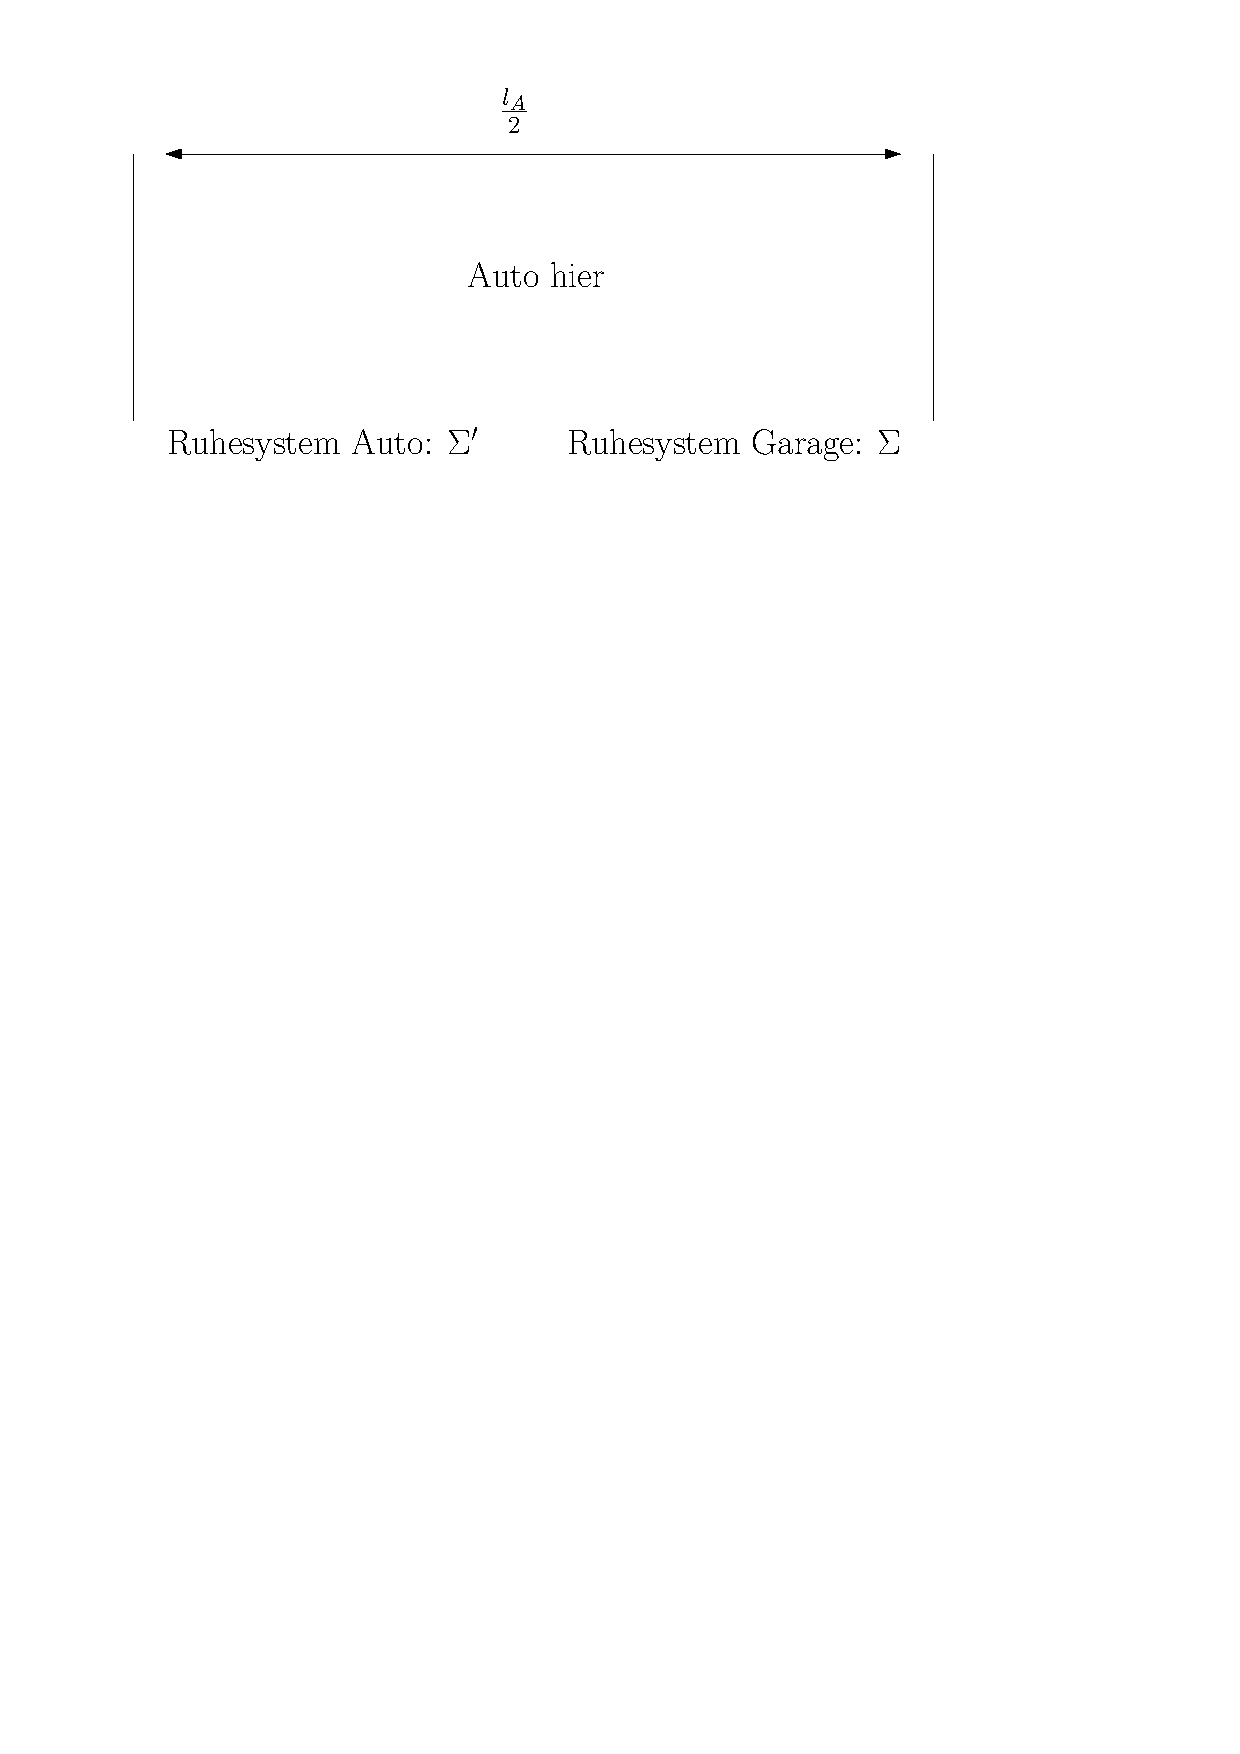
\includegraphics{figures/ueb11/aufgabe24}
	\caption{Aufgabe 24}
	\label{fig:ueb11_aufgabe24}
\end{figure}

Wir setzen $r = (ct, x, y, z)^T$, $r_0 = (c t_0, x_0 = 0)^T$ und $r_1 = (c t_1, x_1 = l_A)^T$ (im Ruhesystem $\Sigma$). Wichtig bei Längenmessung: Beide Endpunkten zum selben Zeitpunkt messen. Wie sieht $r$ in $\Sigma'$ aus? Ausrechnen:
\[
	r' = \Lambda(\vec{v}) r = \begin{pmatrix}
		\gamma & -\gamma \beta \\
		-\gamma \beta & \gamma
	\end{pmatrix}
	\mvec{ct \\ x}
	= \begin{pmatrix}
		\gamma (ct - \beta x) \\
		\gamma (-\beta ct + x)
	\end{pmatrix}
	\text{.}
\]
	
Wenn man das mit $r_0$ bzw. $r_1$ macht, führt das auf die Gleichungen
\[
	\left\{
	\begin{array}{l}
		c t'_0 = \gamma(ct_0 - \beta x_0) \\
		x'_0 = \gamma(-\beta c t_0 + x_0) 	
	\end{array}
	\right.
	\quad \text{ und } \quad
	\left\{
	\begin{array}{l}
		c t'_1 = \gamma(ct_1 - \beta x_1) \\
		x'_1 = \gamma(-\beta c t_1 + x_1) 	
	\end{array}
	\right.
	\text{.}
\]
	
Jetzt fordern wir $c t'_0 = c t'_1$ und damit $\gamma (ct_0 - \beta x_0) = \gamma (c t_1 - \beta x_1)$, also $c (t_1 - t_0) = \beta (x_1 - x_0)$. Es folgt 	
\begin{align*}
	l'_A &= x'_1 = x'_0 = \gamma (- \beta c (t_1 - t_0) + (x_1 - x_0))
	= \gamma (- \beta^2 (x_1 - x_0) + (x_1 - x_0)) \\
	&= \gamma \underbrace{(1 - \beta^2)}_{\frac{1}{\gamma^2}} l_A = \frac{1}{\gamma} l_A
	\text{.}
\end{align*}
Der Term wird als relativistische Längenkontraktion bezeichnet. Für die Aufgabe muss gelten: $\frac{l'_A}{l_A} = \sqrt{1 - \beta^2}$, also $\beta = \sqrt{1 - \left( \frac{l'_A}{l_A} \right)^2}$. Es folgt für $v$:
\[
	v = \sqrt{1 - \left( \frac{l'_A}{l_A} \right)^2} c = \sqrt{\frac{3}{4}} c = \frac{\sqrt{3}}{2} c
		\text{.}
\]

\section*{Aufgabe 25}

Myonen werden in $11 \si{km}$ Höhe erzeugt und haben eine Halbwertszeit $\tau_\mu = 2 \cdot 10^{-6} \si{s}$ und eine Geschwindigkeit von $v \approx c$.

Ohne relativistische Rechnung können sie also einen Weg $\Delta s = c \tau = 3 \cdot 10^5 \si{\frac{km}{s}} 2 \cdot 10^{-6} = 0.6 \si{km}$ zurücklegen und würden die Erdoberfläche somit nicht erreichen.

Nun relativistisch rechnen: System der Myonen sei $\Sigma$ und wir setzen $x_0 = (0, 0)^T$ und $x_1 = (c \tau, 0)^T$. System der Erde sei $\Sigma'$ und wir setzen analog $x'_0 = (0, h'_0)^T$ und $x'_1 = (ct, h'_1)^T$. 

Es ist
\[
	(x'_1 - x'_0) = \begin{pmatrix}
		\gamma & -\gamma \beta \\
		-\gamma \beta & \gamma
	\end{pmatrix}
	(x_1 - x_0)
	\text{,}
\]
also
\[
	\mvec{ct \\ h'_1 - h'_0} = \begin{pmatrix}
		\gamma & -\gamma \beta \\
		-\gamma \beta & \gamma
	\end{pmatrix}
	\mvec{c \tau \\ 0}
	\text{.}
\]
Für die Zeit gilt somit $ct = \gamma c \tau$. Das ist die Zeitdilatation: $t = \gamma \tau$ ($\gamma > 1$). Für die Höhe gilt:
\begin{align*}
	&~ h'_1 - h'_0 = - \gamma \beta c \tau \\
	\Longrightarrow &~ (h'_1 - h'_0)^2 = \frac{\beta^2}{1 - \beta^2} c^2 \tau^2 \\
	\Longleftrightarrow &~ (h'_1 - h'_0)^2 (1 - \beta^2) = \beta^2 c^2 \tau^2 \\
	\Longleftrightarrow &~ \beta^2 ((h'_1 - h'_0)^2 + c^2 \tau^2) = (h'_1 - h'_0)^2 \\
	\Longleftrightarrow &~ \beta^2 = \frac{(h'_1 - h'_0)^2}{(h'_1 - h'_0) + c^2 \tau^2} = \frac{1}{1 + \frac{c^2 \tau^2}{(h'_1 - h'_0)^2}} \\
	\Longrightarrow &~ \beta = \left( 1 + \frac{c^2 \tau^2}{(h'_1 - h'_0)^2} \right)^{- \frac{1}{2}}
	= \left( 1 + \frac{2 \cdot 10^{-6} s 3 \cdot 10^5 \si{\frac{km}{s}}}{(11 \si{km} - 1.5 \si{km})^2} \right)^{-\frac{1}{2}}
	\approx 0.998
	\text{.}
\end{align*}